% !TeX spellcheck = en_US
%\documentclass[11pt,a4paper]{article}
\documentclass[11pt
  , a4paper
  , article
  , oneside
%  , twoside
%  , draft
]{memoir}

\usepackage{control}
\usepackage{kotex}
\usepackage[numbers]{natbib}
%\usepackage[pdftex]{graphicx}
%\DeclareGraphicsExtensions{.pdf,.png,.jpg}
\begin{document}

\newcommand{\technumber}{
  Digital Signal Processing using MATLAB\\
  Document 1: 2016-03-26}
\title{\textbf{Digital Signal Processing: 실습 10 \\
		제5장 이산 푸리에 변환 \\}}

\author{이상일\thanks{silee7103@ibs.re.kr} \\

  학번: 201460437\\
  Computer Engineering, Chungnam National University 
}
\date{\today}

\renewcommand{\maketitlehooka}{\begin{flushright}\textsf{\technumber}\end{flushright}}
%\renewcommand{\maketitlehookb}{\centering\textsf{\subtitle}}
%\renewcommand{\maketitlehookc}{C}
%\renewcommand{\maketitlehookd}{D}

\maketitle

\begin{abstract}
MATLAB을 사용한 Digital Signal Processing에 대한 실습과제에 대한 Documents를 구성한다.
\end{abstract}


\chapter{Example 5-4:}
주어진 식은 에일리어싱 공식에 따라서,

\begin {equation}
\tilde{x_2}(n) = \sum_{r=-\infty}^{\infty} x_1(n-4r) \nonumber
\end {equation}

따라서, x(4)은 x(0)로 에일리어싱되고, x(5)는 x(1)롤 에일리어싱 되어,
\begin {equation}
\tilde{x_2}(n) = {\{...,8,6,4,3,\underline{8},6,4,3,8,6,4,3,...\}} \nonumber
\end {equation}


\chapter{Example 5-5:}

\begin{lstlisting}[style=termstyle]
% Example 5-5

N = 5; k = 0:1:N-1;
wk = 2*pi*k/N;
zk = exp(j*wk);
Xk = (zk)./(zk-0.7);
xn = real(idfs(Xk,N));

xtilde = xn'* ones(1,8); xtilde = (xtilde(:))';
subplot(2,2,1); stem(0:39,xtilde);axis([0,40,-0.1,1.5])
xlabel('n'); ylabel('xtilde(n)'); title('N=5')

N = 10;
k = 0:1:N-1;
wk = 2*pi*k/N;
zk = exp(j*wk);
Xk = (zk)./(zk-0.7);
xn = real(idfs(Xk,N));

xtilde = xn'* ones(1,4); xtilde = (xtilde(:))';
subplot(2,2,2); stem(0:39,xtilde);axis([0,40,-0.1,1.5])

xlabel('n'); ylabel('xtilde(n)'); title('N=10')

N = 20;
k = 0:1:N-1;
wk = 2*pi*k/N;
zk = exp(j*wk);
Xk = (zk)./(zk-0.7);
xn = real(idfs(Xk,N));
xtilde = xn'* ones(1,2); xtilde = (xtilde(:))';
subplot(2,2,3); stem(0:39,xtilde);axis([0,40,-0.1,1.5])

xlabel('n'); ylabel('xtilde(n)'); title('N=20')

N = 40;
k = 0:1:N-1;
wk = 2*pi*k/N;
zk = exp(j*wk);
Xk = (zk)./(zk-0.7);
xn = real(idfs(Xk,N));
subplot(2,2,4); stem(0:39,xn);axis([0,40,-0.1,1.5])
xlabel('n'); ylabel('xtilde(n)'); title('N=40')

\end{lstlisting}

\begin{figure}[h!]
	\centering
	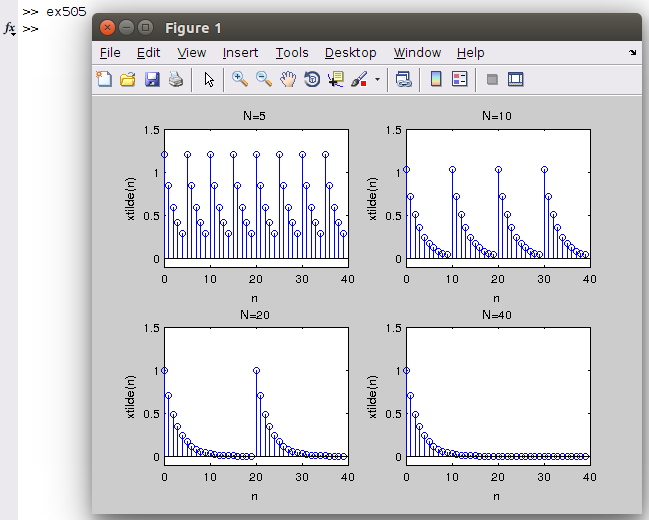
\includegraphics[width=0.6\textwidth,height=0.4\textwidth]{./images/ex505.png}
	\caption{Example 5.5 Result}
	\label{fig:Example 5.5 Result}
\end{figure}

\chapter{Example 5-6:}
\subsection{Example 5-6a}
\begin{lstlisting}[style=termstyle]
% Example 5-6
x = [1,1,1,1];
% a
w = [0:1:500]*2*pi/500;
[H] = freqz(x,1,w);
magH = abs(H); phaH = angle(H); phaH(126)=-47.5841*pi/180;
subplot(2,1,1); plot(w/pi,magH); grid
xlabel('frequency in pi units');
ylabel('|X|'); title('Magnitude of the DTFT')
subplot(2,1,2); plot(w/pi,phaH/pi*180); grid
xlabel('frequency in pi units');
ylabel('Degrees'); title('Angle of the DTFT')
\begin{figure}[h!]
	\centering
	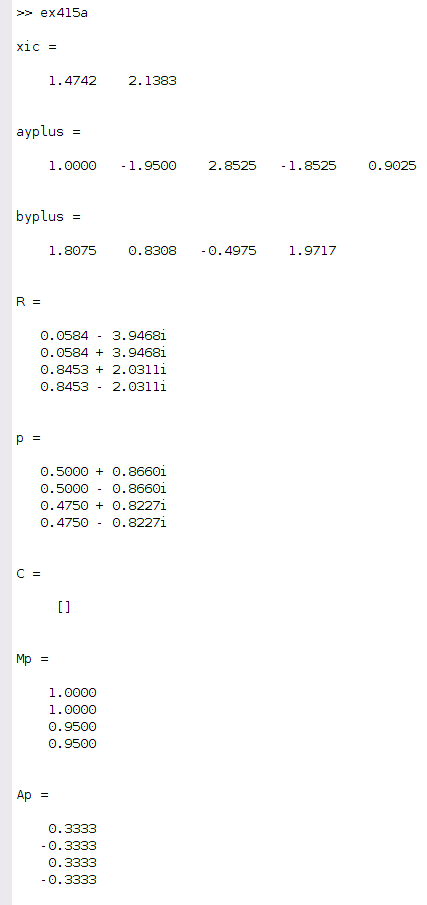
\includegraphics[width=0.6\textwidth,height=0.4\textwidth]{./images/ex415a.png}
	\caption{Example 4.15a Result}
	\label{fig:Example 4.15a Result}
\end{figure}

\subsection{4-15b}
\begin{lstlisting}[style=termstyle]
Example 4.15b

n = [0:7]; x = cos(pi*n/3); y = filter(b,a,x,xic)
A = real(2*R(1)); B = imag(2*R(2)); C = real(2*R(3)); D = imag(2*R(4));

y = A*cos(pi*n/3) + B*sin(pi*n/3) + ((0.95).^n).*(C*cos(pi*n/3)+D*sin(pi*n/3))
\end{lstlisting}

\begin{figure}[h!]
	\centering
	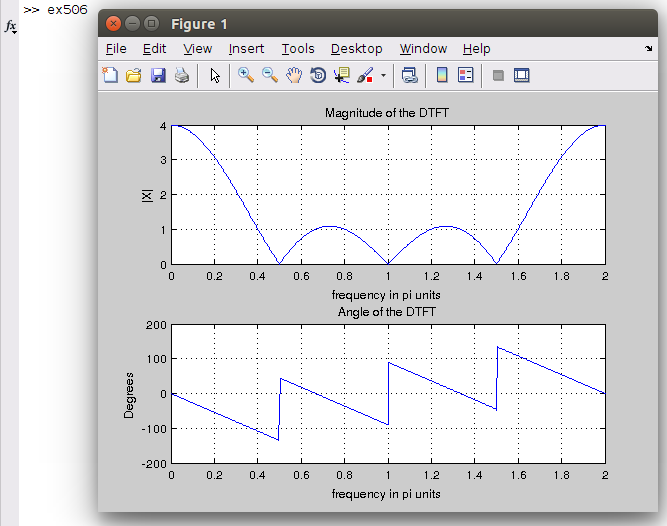
\includegraphics[width=0.5\textwidth,height=0.4\textwidth]{./images/ex506.png}
	\caption{Example 5.6a Result}
	\label{fig:Example 5.6a Result}
\end{figure}

\subsection{Example 5-6a}
\begin{lstlisting}[style=termstyle]
x = [1,1,1,1];

% b
N = 4; w1 = 2*pi/N; k = 0:N-1;
X = dft(x,N);
magX = abs(X), phaX = angle(X)*180/pi
subplot(2,1,1);plot(w*N/(2*pi),magH,'--'); 
axis([-0.1,4.1,-1,5]); hold on
stem(k,magX);
xlabel('k');
ylabel('|X(k)|'); title('Magnitude of the DFT: N=4')

subplot(2,1,2);plot(w*N/(2*pi),phaH*180/pi,'--');
axis([-0.1,4.1,-200,200]);
stem(k,phaX);
xlabel('k');
ylabel('Degrees'); title('Angle of the DFT: N=4')

\end{lstlisting}

\begin{figure}[h!]
	\centering
	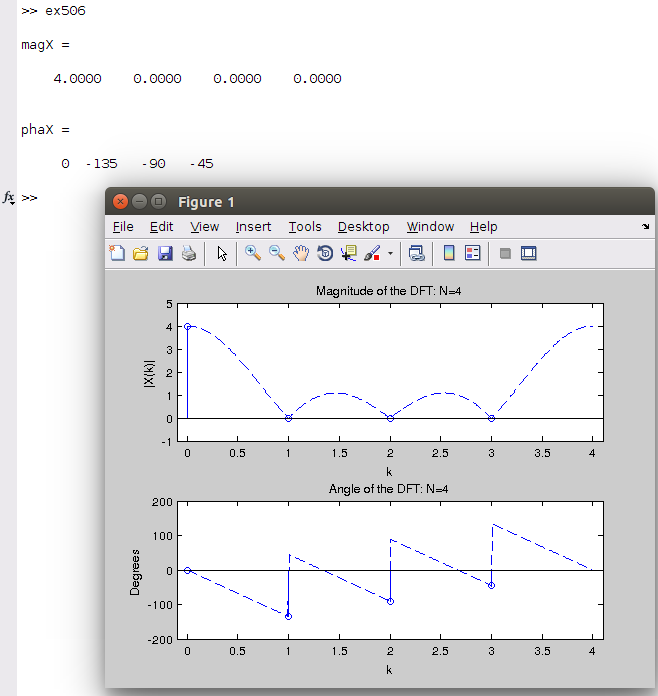
\includegraphics[width=0.5\textwidth,height=0.4\textwidth]{./images/ex506b.png}
	\caption{Example 5.6b Result}
	\label{fig:Example 5.6b Result}
\end{figure}

\chapter{Example 5-7:}
\begin{lstlisting}[style=termstyle]
% Example 5-7
x = [1,1,1,1];
% a
w = [0:1:500]*2*pi/500;
[H] = freqz(x,1,w);
magH = abs(H); phaH = angle(H); phaH(126)=-47.5841*pi/180;

% b
N = 8; w1 = 2*pi/N; k = 0:N-1;
x = [x, zeros(1,4)];
X = dft(x,N);
magX = abs(X), phaX = angle(X)*180/pi
subplot(2,1,1);plot(w*N/(2*pi),magH,'--'); 
axis([-0.1,8.1,-1,5]); hold on
stem(k,magX);
xlabel('k');
ylabel('|X(k)|'); title('Magnitude of the DFT: N=8')

hold off
subplot(2,1,2);plot(w*N/(2*pi),phaH*180/pi,'--');
axis([-0.1,8.1,-200,200]); hold on
stem(k,phaX);
xlabel('k');
ylabel('Degrees'); title('Angle of the DFT: N=8');pause

% c
N = 16; w1 = 2*pi/N; k = 0:N-1;
x = [x, zeros(1,8)];
X = dft(x,N);
magX = abs(X), phaX = angle(X)*180/pi
subplot(2,1,1);plot(w*N/(2*pi),magH,'--'); 
axis([-0.1,16.1,-1,5]); hold on
stem(k,magX);
xlabel('k');
ylabel('|X(k)|'); title('Magnitude of the DFT: N=16')
hold off
subplot(2,1,2);plot(w*N/(2*pi),phaH*180/pi,'--');
axis([-0.1,16.1,-200,200]); hold on
stem(k,phaX);

xlabel('k');
ylabel('Degrees'); title('Angle of the DFT: N=16')

\end{lstlisting}

\begin{figure}[h!]
	\centering
	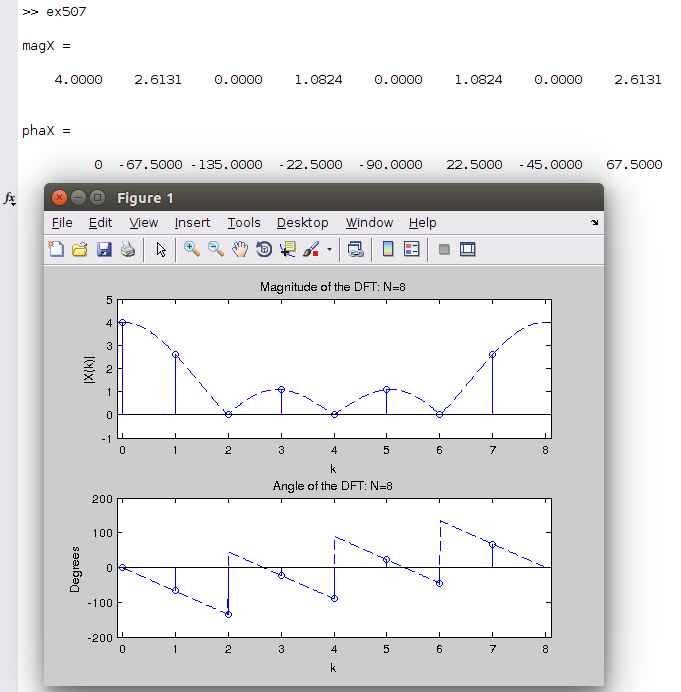
\includegraphics[width=0.5\textwidth,height=0.4\textwidth]{./images/ex507a.png}
	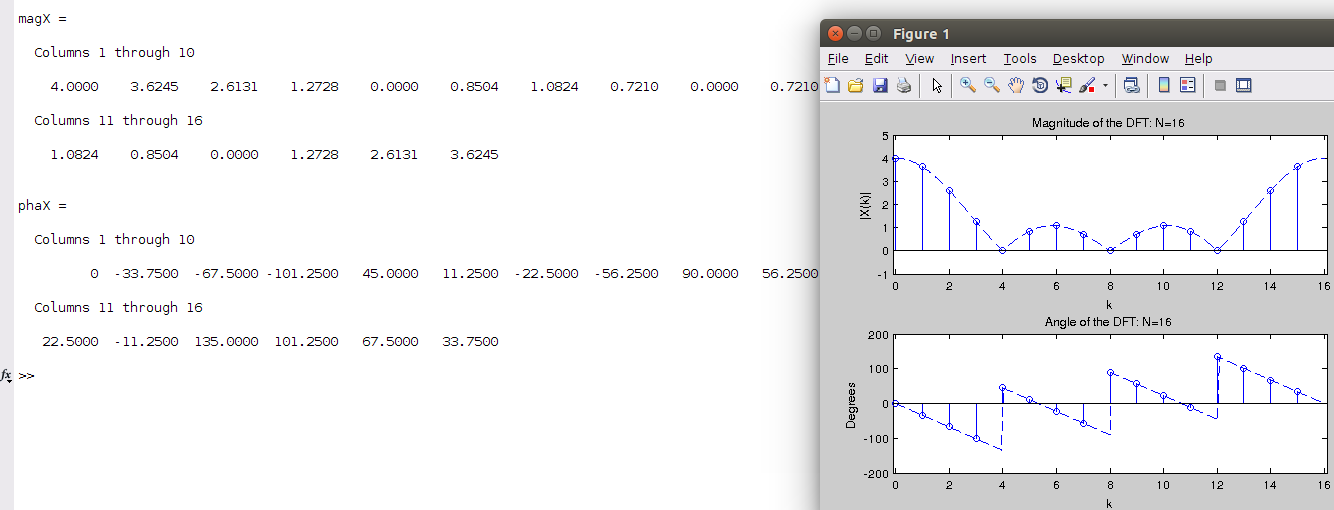
\includegraphics[width=0.5\textwidth,height=0.4\textwidth]{./images/ex507b.png}
	\caption{Example 5.7 Result}
	\label{fig:Example 5.7 Result}
\end{figure}

\chapter{Example 5-8:}
\subsection{Example 5-8a}
\begin{lstlisting}[style=termstyle]
% Example 5-8a

n=[0:1:99];
x=cos(0.48*pi*n)+cos(0.52*pi*n);
subplot(2,1,1);stem(n,x);title('signal x(n), 0 <= n <= 99');xlabel('n')
axis([0,100,-2.5,2.5])
X=fft(x);magX=abs(X(1:1:51));
k=0:1:50;w=2*pi/100*k;
subplot(2,1,2);plot(w/pi,magX);title('DTFT Magnitude');xlabel('frequency in pi units')
axis([0,1,0,60])

disp('Press RETURN to continue');pause;

% Spectrum based on the first 10 samples of x(n)
n1=[0:1:9];y1=x(1:1:10);
subplot(2,1,1);stem(n1,y1);title('signal x(n), 0 <= n <= 9');xlabel('n')
axis([0,10,-2.5,2.5])
Y1=fft(y1);magY1=abs(Y1(1:1:6));
k1=0:1:5;w1=2*pi/10*k1;
subplot(2,1,2);stem(w1/pi,magY1);title('Samples of DTFT Magnitude');
xlabel('frequency in pi units')
axis([0,1,0,10])

disp('Press RETURN to continue');pause;

% High density spectrum (100 samples) based on the first 10 samples of x(n)
n3=[0:1:99];y3=[x(1:1:10) zeros(1,90)];
subplot(2,1,1);stem(n3,y3);title('signal x(n), 0 <= n <= 9 + 90 zeros');xlabel('n')
axis([0,100,-2.5,2.5])
Y3=fft(y3);magY3=abs(Y3(1:1:51));
k3=0:1:50;w3=2*pi/100*k3;
subplot(2,1,2);plot(w3/pi,magY3);title('DTFT Magnitude');xlabel('frequency in pi units')
axis([0,1,0,10])
disp('Press RETURN to continue');pause;


\end{lstlisting}

\begin{figure}[h!]
	\centering
	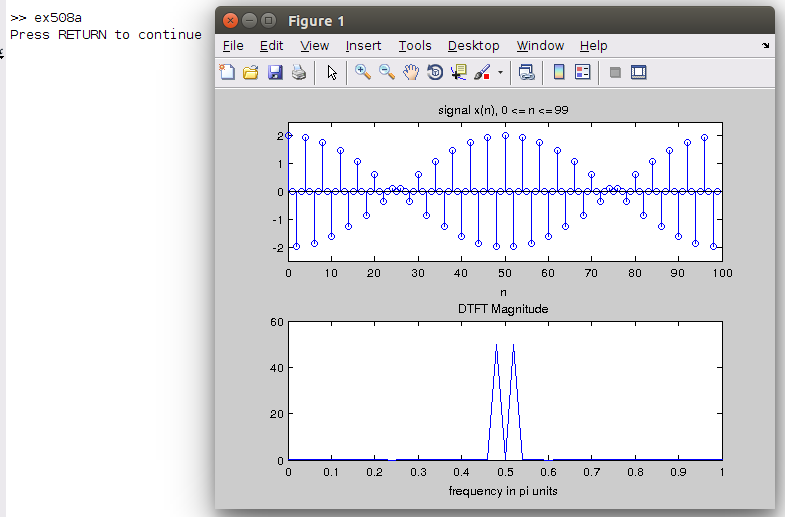
\includegraphics[width=0.5\textwidth,height=0.4\textwidth]{./images/ex508a.png}
	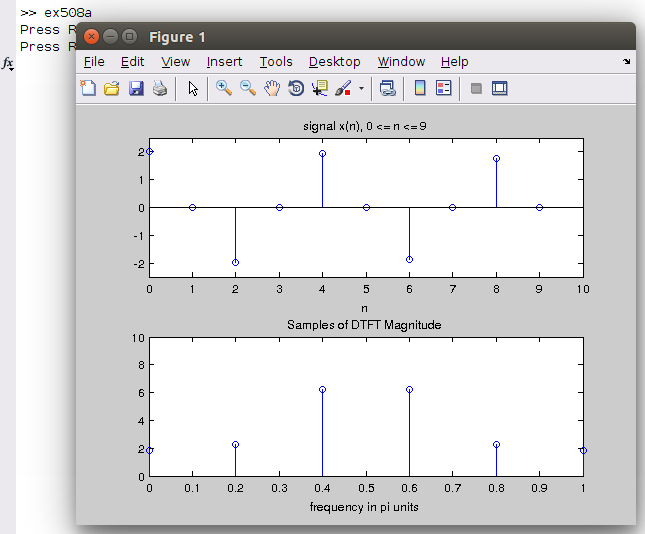
\includegraphics[width=0.5\textwidth,height=0.4\textwidth]{./images/ex508b.png}
	\caption{Example 5.8a Result}
	\label{fig:Example 5.8a Result}
\end{figure}

\clearpage

\subsection{Example 5-8b}
\begin{lstlisting}[style=termstyle]
% Example 5-8b

n = [0:1:99]; x = cos(0.48*pi*n)+cos(0.52*pi*n);

n1 = [0:1:9]; y1 = x(1:1:10);
subplot(2,3,1); stem(n1,y1);
title('x(n), 0 <= n <= 9');xlabel('n');
axis([0,10,-2.5,2.5]); set(gca,'fontsize',10)
Y1 = fft(y1); magY1 = abs(Y1(1:1:6));
k1 = 0:1:5; w1 = 2*pi/10*k1;
subplot(2,3,4);stem(w1/pi,magY1);title('Samples of DTFT Magnitude');
xlabel('frequency in pi units'); axis([0,1,0,10]); set(gca,'fontsize',10)

% High density spectrum (100 samples) based on the first 10 samples of x(n)
n2= [0:1:99]; y2 = [x(1:1:10) zeros(1,90)];
subplot(2,3,2); stem(n2,y2); title('x(n), 0 <= n <= 9 + 90 zeros'); xlabel('n')
axis([0,100,-2.5,2.5]); set(gca,'fontsize',10)
Y2 = fft(y2);magY2=abs(Y2(1:1:51));
k2 = 0:1:50; w2 = 2*pi/100*k2;
subplot(2,3,5); plot(w2/pi,magY2); title('DTFT Magnitude'); xlabel('frequency in pi units')
axis([0,1,0,10]); set(gca,'fontsize',10)

% High resolution spectrum based on 100 samples of the signal x(n)
subplot(2,3,3); stem(n,x); title('x(n), 0 <= n <= 99');xlabel('n')
axis([0,100,-2.5,2.5]); set(gca,'fontsize',10)
X = fft(x); magX=abs(X(1:1:51));
k = 0:1:50; w = 2*pi/100*k;
subplot(2,3,6);plot(w/pi,magX);title('DTFT Magnitude');xlabel('frequency in pi units')
axis([0,1,0,60]); set(gca,'fontsize',10)

\end{lstlisting}

\begin{figure}[h!]
	\centering
	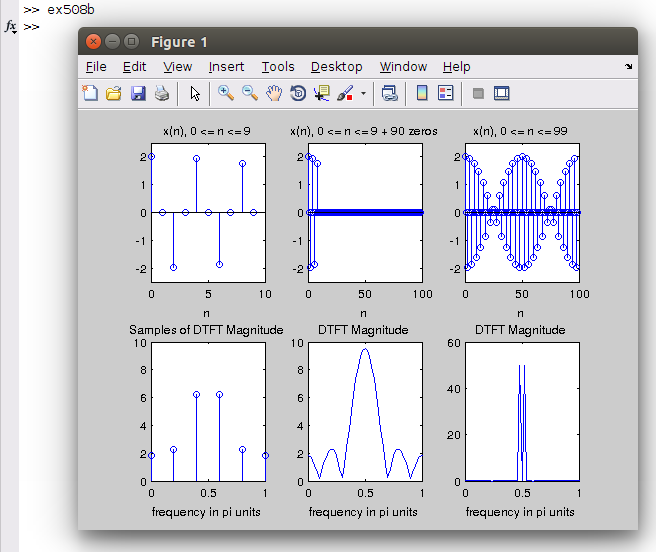
\includegraphics[width=0.5\textwidth,height=0.4\textwidth]{./images/ex508c.png}
	\caption{Example 5.8b Result}
	\label{fig:Example 5.8b Result}
\end{figure}


\chapter{Example 5-9:}
\subsection{Example 5-9a}
\begin{lstlisting}[style=termstyle]
% Example 5-9a

% a)
n = 0:10; x = 10*(0.8) .^ n;
y = x(mod(-n,11)+1);
subplot(2,1,1); stem(n,x); title('Original sequence')
xlabel('n'); ylabel('x(n)'); axis([-0.5,10.5,-1,11])
subplot(2,1,2); stem(n,y); title('Circularly folded sequence')
xlabel('n'); ylabel('x(-n mod 11)'); axis([-0.5,10.5,-1,11])
\end{lstlisting}

\begin{figure}[h!]
	\centering
	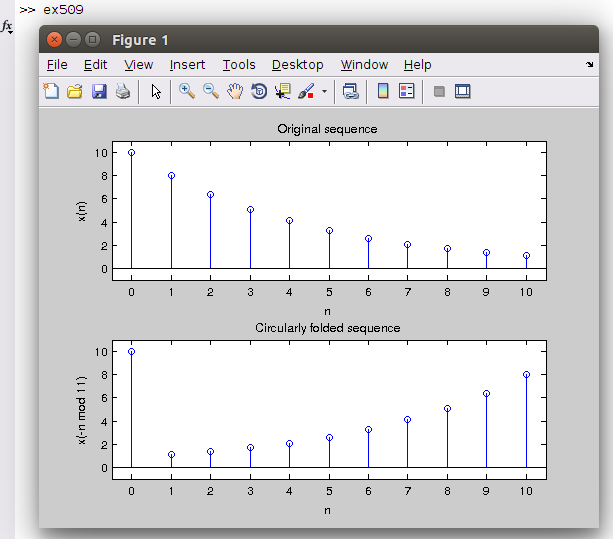
\includegraphics[width=0.5\textwidth,height=0.4\textwidth]{./images/ex509a.png}
	\caption{Example 5.9a Result}
	\label{fig:Example 5.9a Result}
\end{figure}

\subsection{Example 5-9a}
\begin{lstlisting}[style=termstyle]
% Example 5-9b

% b) verify property
X = dft(x,11); Y = dft(y,11);
subplot(2,2,1); stem(n,real(X)); axis([-0.5,10.5,-5,50])
title('Real{DFT[x(n)]}'); xlabel('k');
subplot(2,2,2); stem(n,imag(X)); axis([-0.5,10.5,-20,20])
title('Imag{DFT[x(n)]}'); xlabel('k');
subplot(2,2,3); stem(n,real(Y)); axis([-0.5,10.5,-5,50])
title('Real{DFT[x((-n))11]}'); xlabel('k');
subplot(2,2,4); stem(n,imag(Y)); axis([-0.5,10.5,-20,20])
title('Imag{DFT[x((-n))11]}'); xlabel('k');
\end{lstlisting}

\begin{figure}[h!]
	\centering
	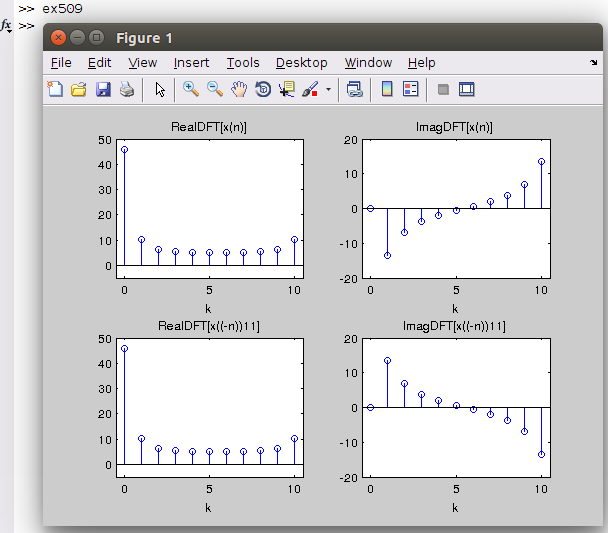
\includegraphics[width=0.5\textwidth,height=0.4\textwidth]{./images/ex509b.png}
	\caption{Example 5.9b Result}
	\label{fig:Example 5.9b Result}
\end{figure}

\chapter{Example 5-10:}
\subsection{Example 5-10a}
\begin{lstlisting}[style=termstyle]
% Example 5-10

% a) plot xec(n) and xoc(n)
n = 0:10; x = 10*(0.8) .^ n;
[xec,xoc] = circevod(x);
subplot(2,1,1); stem(n,xec); title('Circular-even component')
xlabel('n'); ylabel('xec(n)'); axis([-0.5,10.5,-1,11])
subplot(2,1,2); stem(n,xoc); title('Circular-odd component')
xlabel('n'); ylabel('xoc(n)'); axis([-0.5,10.5,-4,4])
pause;
\end{lstlisting}

\begin{figure}[h!]
	\centering
	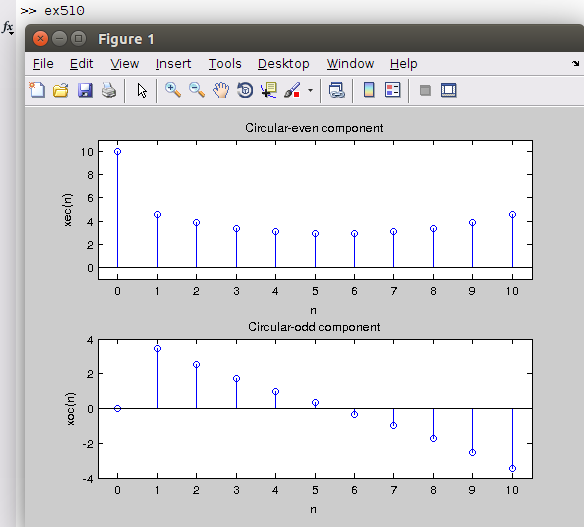
\includegraphics[width=0.5\textwidth,height=0.4\textwidth]{./images/ex510a.png}
	\caption{Example 5.10a Result}
	\label{fig:Example 5.10a Result}
\end{figure}

\subsection{Example 5-10b}
\begin{lstlisting}[style=termstyle]
% Example 5-10b

% b) verify property
X = dft(x,11); Xec = dft(xec,11); Xoc = dft(xoc,11);
subplot(2,2,1); stem(n,real(X)); axis([-0.5,10.5,-5,50])
title('Real{DFT[x(n)]}'); xlabel('k');
subplot(2,2,2); stem(n,imag(X)); axis([-0.5,10.5,-20,20])
title('Imag{DFT[x(n)]}'); xlabel('k');
subplot(2,2,3); stem(n,real(Xec)); axis([-0.5,10.5,-5,50])
title('DFT[xec(n)]'); xlabel('k');
subplot(2,2,4); stem(n,imag(Xoc)); axis([-0.5,10.5,-20,20])
title('DFT[xoc(n)]'); xlabel('k');

\end{lstlisting}

\begin{figure}[h!]
	\centering
	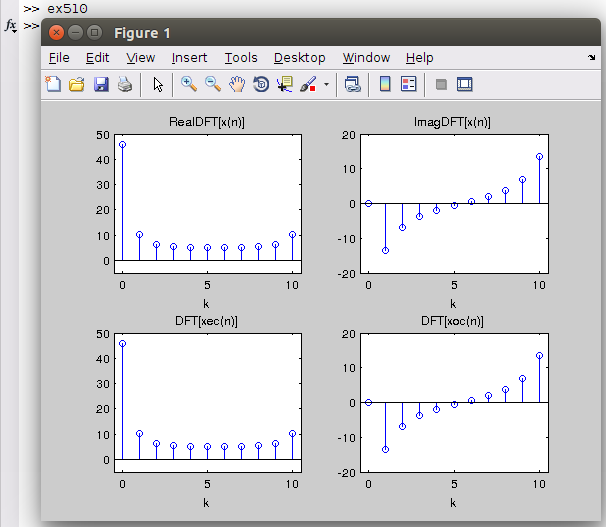
\includegraphics[width=0.5\textwidth,height=0.4\textwidth]{./images/ex510b.png}
	\caption{Example 5.10b Result}
	\label{fig:Example 5.10b Result}
\end{figure}


\chapter{Example 5-11:}
\subsection{Example 5-11a}
\begin{lstlisting}[style=termstyle]
% Example 5-11


% a) plot x((n+4))11
n = 0:10; x = 10*(0.8) .^ n;
n1 = -11:21; x1 = [zeros(1,11), x, zeros(1,11)];
subplot(2,2,1); stem(n1,x1); title('Original x(n)')
xlabel('n'); axis([-6,17,-1,11])
x2 = [x, x, x];
subplot(2,2,3); stem(n1,x2); title('Periodic extention')
xlabel('n'); axis([-6,17,-1,11])
x3 = [x2(4+1:33), x(1:4)];
subplot(2,2,2); stem(n1,x3); title('Periodic shift')
xlabel('n'); axis([-6,17,-1,11])
x4 = x3 .* [zeros(1,11), ones(1,11), zeros(1,11)];
subplot(2,2,4); stem(n1,x4); title('Circular shift')
xlabel('n'); axis([-6,17,-1,11])

pause;
\end{lstlisting}

\clearpage
\begin{figure}[h!]
	\centering
	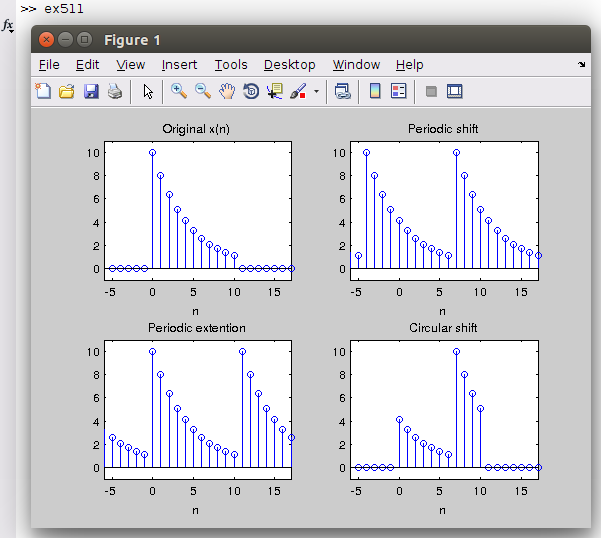
\includegraphics[width=0.5\textwidth,height=0.3\textwidth]{./images/ex511.png}
	\caption{Example 5.11a Result}
	\label{fig:Example 5.11a Result}
\end{figure}


\subsection{Example 5-11b}
\begin{lstlisting}[style=termstyle]
% Example 5-11b

% b) plot x((n-3))15
n = 0:10; x = [10*(0.8) .^ n zeros(1,4)];
n1 = -15:29; x1 = [zeros(1,15), x, zeros(1,15)];
subplot(2,2,1); stem(n1,x1); title('Original x(n)')
xlabel('n'); axis([-9,25,-1,11])
x2 = [x, x, x];
subplot(2,2,3); stem(n1,x2); title('Periodic extention')
xlabel('n'); axis([-9,25,-1,11])
x3 = [x2(43:45),x2(1:42)];
subplot(2,2,2); stem(n1,x3); title('Periodic shift')
xlabel('n'); axis([-9,25,-1,11])
x4 = x3 .* [zeros(1,15), ones(1,15), zeros(1,15)];
subplot(2,2,4); stem(n1,x4); title('Circular shift')
xlabel('n'); axis([-9,25,-1,11])

\end{lstlisting}

\begin{figure}[h!]
	\centering
	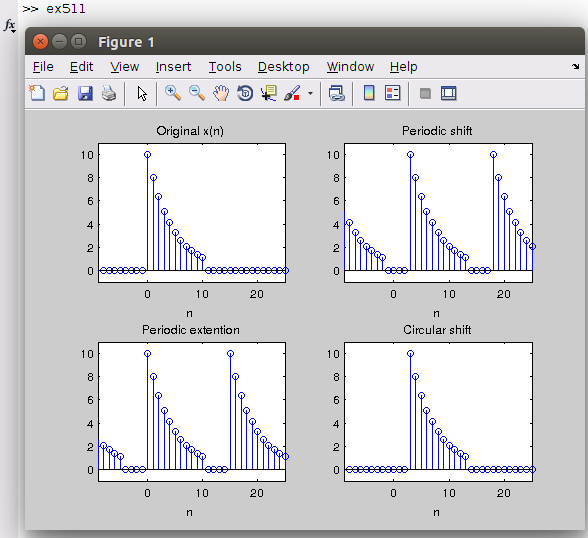
\includegraphics[width=0.5\textwidth,height=0.3\textwidth]{./images/ex511b.png}
	\caption{Example 5.11b Result}
	\label{fig:Example 5.11b Result}
\end{figure}

\clearpage

\chapter{Example 5-12:}
\begin{lstlisting}[style=termstyle]
% Example 5-12

n = 0:10; x = 10*(0.8) .^ n;
y = cirshftt(x,6,15); 
n = 0:14; x = [x, zeros(1,4)];
subplot(2,1,1); stem(n,x); title('Original sequence')
xlabel('n'); ylabel('x(n)'); axis([-1,15,-1,11])
subplot(2,1,2); stem(n,y); 
title('Circularly shifted sequence, N=15')
xlabel('n'); ylabel('x((n-6) mod 15)'); 
axis([-1,15,-1,11])
\end{lstlisting}
\begin{figure}[h!]
	\centering
	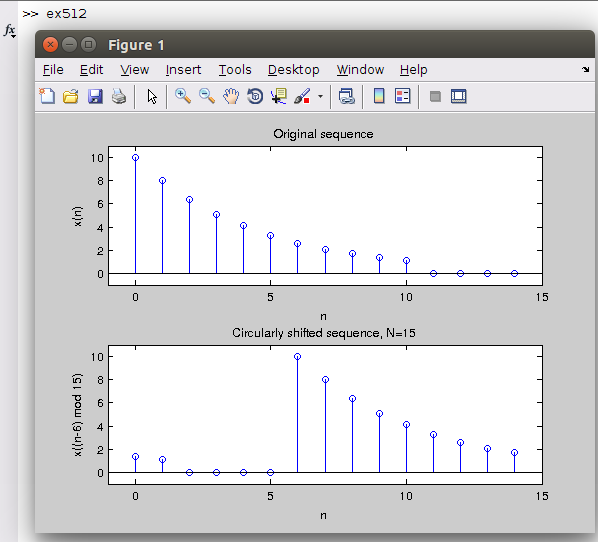
\includegraphics[width=0.5\textwidth,height=0.4\textwidth]{./images/ex512.png}
	\caption{Example 5.12 Result}
	\label{fig:Example 5.12 Result}
\end{figure}

\chapter{Example 5-14:}
\begin{lstlisting}[style=termstyle]
% Example 5-14
x1 = [1,2,2]; x2 = [1,2,3,4];
y = circonvt(x1,x2,4)
\end{lstlisting}

\begin{figure}[h!]
	\centering
	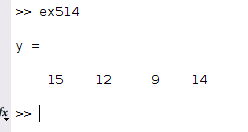
\includegraphics[width=0.5\textwidth,height=0.2\textwidth]{./images/ex514.png}
	\caption{Example 5.14 Result}
	\label{fig:Example 5.14 Result}
\end{figure}

\chapter{Common: M-Functions}
dft.m:
\begin{lstlisting}[style=termstyle]
function [Xk] = dft(xn,N)
% Computes Discrete Fourier Transform
% -----------------------------------
% [Xk] = dft(xn,N)
% Xk = DFT coeff. array over 0 <= k <= N-1
% xn = N-point finite-duration sequence
%  N = Length of DFT

n = [0:1:N-1];                       % row vector for n
k = [0:1:N-1];                       % row vecor for k
WN = exp(-j*2*pi/N);                 % Wn factor
nk = n'*k;                           % creates a N by N matrix of nk values
WNnk = WN .^ nk;                     % DFT matrix
Xk = xn * WNnk;                      % row vector for DFT coefficients
\end{lstlisting}

circevod.m:
\begin{lstlisting}[style=termstyle]
function [xec, xoc] = circevod(x)
% signal decomposition into circular-even and circular-odd parts
% --------------------------------------------------------------
% [xec, xoc] = circecod(x)

if any(imag(x) ~= 0)
error('x is not a real sequence')
end

N = length(x); n = 0:(N-1);
xec = 0.5*(x + x(mod(-n,N)+1));
xoc = 0.5*(x - x(mod(-n,N)+1));
\end{lstlisting}

cirshftt.m:
\begin{lstlisting}[style=termstyle]
function y = cirshftt(x,m,N)
% Circular shift of m samples wrt size N in sequence x: (time domain)
% -------------------------------------------------------------------
% [y] = cirshftt(x,m,N)
% y = output sequence containing the circular shift
% x = input sequence of length <= N
% m = sample shift
% N = size of circular buffer
%  Method: y(n) = x((n-m) mod N)

% Check for length of x
if length(x) > N
error('N must be >= the length of x')
end

x = [x zeros(1,N-length(x))];
n = [0:1:N-1];
n = mod(n-m,N);
y = x(n+1);

\end{lstlisting}

circonvt.m:
\begin{lstlisting}[style=termstyle]
function y = circonvt(x1,x2,N)
% N-point circular convolution between x1 and x2: (time-domain)
% -------------------------------------------------------------
% [y] = circonvt(x1,x2,N)
%  y = output sequence containing the circular convolution
% x1 = input sequence of length N1 <= N
% x2 = input sequence of length N2 <= N
%  N = size of circular buffer
%  Method: y(n) = sum (x1(m)*x2((n-m) mod N))

% Check for length of x1
if length(x1) > N
error('N must be >= the length of x1')
end

% Check for length of x2
if length(x2) > N
error('N must be >= the length of x2')
end

x1=[x1 zeros(1,N-length(x1))];
x2=[x2 zeros(1,N-length(x2))];

m = [0:1:N-1];

x2 = x2(mod(-m,N)+1);
H = zeros(N,N);

for n = 1:1:N
H(n,:) = cirshftt(x2,n-1,N);
end

y = x1*H';
\end{lstlisting}

idfs.m:
\begin{lstlisting}[style=termstyle]
function [xn] = idfs(Xk,N)
% Computes Inverse Discrete Fourier Series
% ----------------------------------------
% [xn] = idfs(Xk,N)
% xn = One period of periodic signal over 0 <= n <= N-1
% Xk = DFS coeff. array over 0 <= k <= N-1
%  N = Fundamental period of Xk

n = [0:1:N-1];                       % row vector for n
k = [0:1:N-1];                       % row vecor for k
WN = exp(-j*2*pi/N);                 % Wn factor
nk = n'*k;                           % creates a N by N matrix of nk values
WNnk = WN .^ (-nk);                  % IDFS matrix
xn = (Xk * WNnk)/N;                  % row vector for IDFS values
\end{lstlisting}

\end{document}

